\documentclass{beamer}
\usepackage[utf8]{inputenc}
\usetheme{Madrid}
\title[Object Pooling]{Object Pooling}
\author{Ashiqur Rahman}
\date{July 2019}
\newcommand{\code}[1]{\texttt{#1}}

\begin{document}
\maketitle

\begin{frame}{Table Of Contents}
	\centering
	\tableofcontents
\end{frame}

\section{Intro}
\begin{frame}{Intro}

	The object pool pattern is a software creational design pattern that uses a set of initialized objects kept ready to use – a "pool" – rather than allocating and destroying them on demand
	
\end{frame}

\section{Benefits}
\begin{frame}{Benefits}
	Object pooling can offer a significant performance boost in situations where the cost of initializing a class instance is high and the rate of instantiation and destruction of a class is high – in this case objects can frequently be reused, and each reuse saves a significant amount of time. Object pooling requires resources – memory and possibly other resources, such as network sockets, and thus it is preferable that the number of instances in use at any one time is low, but this is not required.
	The pooled object is obtained in predictable time when creation of the new objects (especially over network) may take variable time. These benefits are mostly true for objects that are expensive with respect to time, such as database connections, socket connections, threads and large graphic objects like fonts or bitmaps.
\end{frame}
	
\begin{frame}{Benefits Continued ..}
	In other situations, simple object pooling (that hold no external resources, but only occupy memory) may not be efficient and could decrease performance.In case of simple memory pooling, the slab allocation memory management technique is more suited, as the only goal is to minimize the cost of memory allocation and deallocation by reducing fragmentation.
\end{frame}

\section{Implementation}
\begin{frame}{Implementation}
Object pools can be implemented in an automated fashion in languages like C++ via smart pointers. In the constructor of the smart pointer, an object can be requested from the pool, and in the destructor of the smart pointer, the object can be released back to the pool. In garbage-collected languages, where there are no destructors (which are guaranteed to be called as part of a stack unwind), object pools must be implemented manually, by explicitly requesting an object from the factory and returning the object by calling a dispose method (as in the dispose pattern). Using a finalizer to do this is not a good idea, as there are usually no guarantees on when (or if) the finalizer will be run. Instead, "try ... finally" should be used to ensure that getting and releasing the object is exception-neutral.

Manual object pools are simple to implement, but harder to use, as they require manual memory management of pool objects.
\end{frame}

\begin{frame}{Implementation C \#}

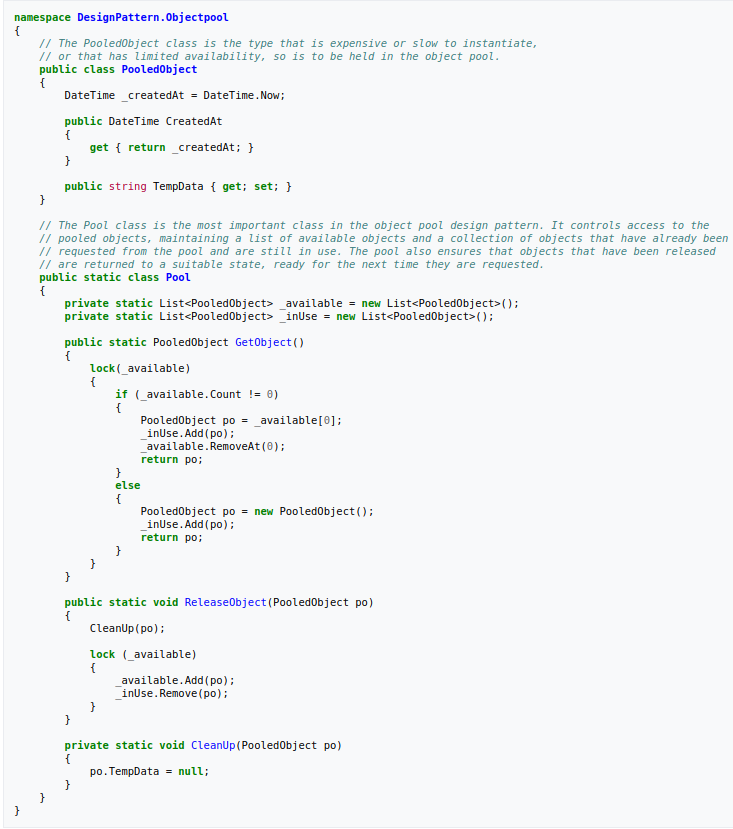
\includegraphics[scale=0.25]{c.png}
\centering
\end{frame}

\end{document}